\documentclass{beamer}

\usepackage{graphicx}
\usepackage{tikz}
\usetikzlibrary{positioning, arrows.meta, calc, backgrounds}
\pgfdeclarelayer{background}
\pgfsetlayers{background,main}
\usepackage{transparent}
\usetheme{Madrid}

\usepackage[style=authoryear]{biblatex}


\makeatletter
\renewcommand{\footnotesize}{\tiny}
\makeatother

\addbibresource{refs/daftar_pustaka.bib}
%Information to be included in the title page:
\title[]
{Presentasi Research Activity}

\subtitle{Deteksi Perubahan Deforestasi Menggunakan Siamese U-Net}

\author[Aldi Pramudya]
{Aldi Pramudya \\ \texttt{G6401231003}}


\institute[IPB]
{
	Program Studi Ilmu Komputer \\
	Sekolah Sains dan Matematika (SSMI) \\
	Institut Pertanian Bogor (IPB University)
}

\date{6 Juni 2026}

% Uncomment and replace with your logo file if needed
% \logo{\includegraphics[height=1cm]{logo-ipb.png}}

\logo{
	\begin{tikzpicture}
		\node[opacity=0.3] {
			
\includegraphics[height=1cm]{./images/ipb_logo.png}
		};
	\end{tikzpicture}
}
\begin{document}
	
	\frame{\titlepage}
	
	\begin{frame}
		\frametitle{Latar Belakang}
		\begin{itemize}
		\item Konversi hutan tropis menjadi perkebunan monokultur telah berlangsung secara masif selama dua dekade terakhir.
		
		\item Pada periode 2002--2024, Kalimantan Barat kehilangan 1{,}4 juta hektare hutan primer basah, setara dengan 33\% dari total kehilangan tutupan pohon, sehingga luas hutan primer basah berkurang sekitar 20\%. \footfullcite{GFW2026}
		
		\item Deteksi perubahan citra satelit merupakan tugas penting dalam \textit{remote sensing} untuk pemantauan lingkungan, penilaian bencana, dan perencanaan perkotaan. Metode \textit{pixel-based} tradisional relatif efisien, tetapi rentan terhadap \textit{noise}, variasi pencahayaan, dan ketidakselarasan geometrik sehingga kurang tangguh pada kondisi nyata. \footfullcite{richards2022remote} \footfullcite{Ali2026}
		\end{itemize}
	\end{frame}

	\begin{frame}
		\frametitle{Latar Belakang (1)}
		\begin{itemize}
		\item \textit{Deep Learning} (DL) telah merevolusi bidang ini dengan memungkinkan pembelajaran fitur secara otomatis. Arsitektur \textit{TransSiamUNet} yang mengombinasikan \textit{Siamese networks}, \textit{U-Net segmentation}, dan \textit{Vision Transformers (ViT)} berhasil mencapai \textit{F-1-score} 0,928 pada dataset LEVIR-CD. \footfullcite{Ali2026}.
		\item Meskipun menjanjikan, arsitektur \textit{TransSiamUNet} memiliki kompleksitas dan kebutuhan sumber daya yang tinggi sehingga kurang efisien pada lingkungan dengan keterbatasan komputasi.
    
		\item Model DL juga cenderung bersifat \textit{black box}, yang dapat mengurangi interpretabilitas dan kepercayaan pengguna, terutama pada aplikasi pemantauan lingkungan.
		\end{itemize}
	\end{frame}
	
	\begin{frame}
		\frametitle{Latar Belakang (2)}
		\begin{itemize}
		\item Penelitian ini mengusulkan pendekatan berbasis DL untuk mendeteksi perubahan deforestasi di Kalimantan menggunakan citra satelit multispektral.
		
		\item Fokus pada pengembangan arsitektur \textit{Siamese U-Net} yang dimodifikasi untuk mencapai keseimbangan antara performa dan efisiensi, serta mengintegrasikan teknik \textit{Explainable Artificial Intelligence} (XAI) guna meningkatkan interpretabilitas model.
		\end{itemize}
	\end{frame}
	
	\begin{frame}
		\frametitle{Jenis Metode Penelitian}
		
		\begin{block}{Metode Penelitian}
			Penelitian ini menggunakan metode penelitian 
			\textbf{kuantitatif} dengan tambahan analisis kualitatif dengan XAI.
		\end{block}
		
		\vspace{0.3cm}
		
		\begin{itemize}
			\item Menggunakan data numerik dari citra satelit multispektral
			\item Mengukur performa model deep learning
			\item Menggunakan metrik evaluasi statistik:
			\begin{itemize}
				\item Intersection over Union (IoU)
				\item Precision
				\item Recall
				\item F1-Score
			\end{itemize}
		\end{itemize}
		
		\vspace{0.3cm}
	\end{frame}
	
	\begin{frame}
		\frametitle{Pengumpulan Data}
		
		\begin{block}{Sumber Data}
			\begin{itemize}
				\item Sentinel-2 Level-2A
				\item Hansen Global Forest Change
			\end{itemize}
		\end{block}
		
		\vspace{0.3cm}
		
		\begin{block}{Metode Pengumpulan}
			\begin{itemize}
				\item Akuisisi data menggunakan Google Earth Engine
				\item Cloud masking
				\item Median compositing
			\end{itemize}
		\end{block}
		
		\textbf{Lingkup penelitian dibatasi pada pulau Kalimantan}.
		
	\end{frame}
	
	\begin{frame}
		\frametitle{Pra-pemrosesan Data (1)}
		
		\begin{itemize}
			\item \textbf{Normalisasi Data}
			\begin{itemize}
				\item Nilai piksel dinormalisasi ke rentang [0,1]
			\end{itemize}
			
			\vspace{0.2cm}
			
			\item \textbf{Tiling Citra}
			\begin{itemize}
				\item Patch berukuran 256 $\times$ 256
				\item Overlap 16px.
			\end{itemize}
			
			\vspace{0.2cm}
			
			\item \textbf{Spatial Split Dataset}
			\begin{itemize}
				\item Train : 70\%
				\item Validation : 15\%
				\item Test : 15\%
			\end{itemize}
		\end{itemize}
		
	\end{frame}
	
	\begin{frame}
		\frametitle{Contoh Tiling Citra}
		\begin{center}
			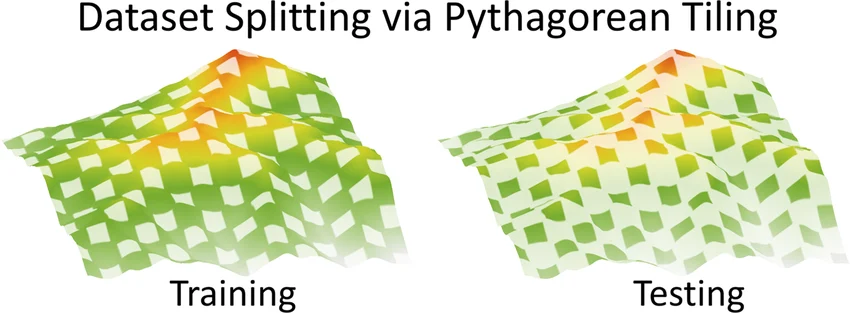
\includegraphics[width=0.8\textwidth]{images/pythagorean_splitting.png}\\
			\vspace{0.15cm}
			\scriptsize
		\end{center}
		\tiny Ilustrasi pembagian data spasial menggunakan \textit{Pythagorean tiling}. Metode ini digunakan untuk membagi data dari wilayah yang dimodelkan secara representatif secara spasial, sehingga variasi karakteristik antara partisi pelatihan dan pengujian tetap terjaga. Dengan \textit{Pythagorean tiling}, dihasilkan pola menyerupai papan catur dengan rasio luas kotak 70/30\%, di mana kotak yang lebih besar digunakan sebagai data pelatihan (\textit{training}) dan kotak yang lebih kecil digunakan sebagai data pengujian (\textit{testing}).\footfullcite{youssef2023landslide}
	\end{frame}
	
	\begin{frame}
		\frametitle{Pra-pemrosesan Data (2)}
		
		\begin{itemize}
			
			\item \textbf{Class Imbalance Handling}
			\begin{itemize}
				\item Area deforestasi lebih sedikit
				\item Menggunakan weighted loss
				\item Kombinasi BCE Loss dan Dice Loss
			\end{itemize}
			
			\vspace{0.2cm}
			
			\item \textbf{Data Augmentation}
			\begin{itemize}
				\item Horizontal flip
				\item Vertical flip
				\item Random rotation
				\item Brightness/contrast adjustment
			\end{itemize}
			
		\end{itemize}
		
	\end{frame}
	
	\begin{frame}
		\frametitle{Arsitektur Model}
		
		\begin{block}{Siamese U-Net}
			Model menggunakan dua encoder identik dengan
			\textit{shared weights} untuk memproses citra
			sebelum (T1) dan sesudah (T2).
		\end{block}
		
		\vspace{0.3cm}
		
		\begin{center}
			%--- scaled picture -------------------------------------------------
			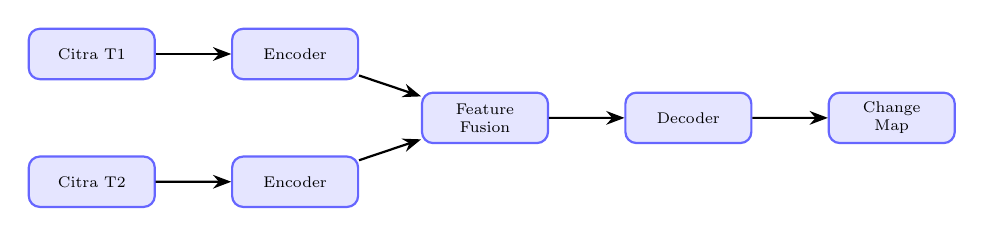
\begin{tikzpicture}[scale=0.8, transform shape,
				node distance=1.2cm,
				block/.style={
					rectangle,
					rounded corners,
					draw=blue!60,
					fill=blue!10,
					thick,
					minimum width=2.0cm,
					minimum height=0.8cm,
					align=center,
					font=\scriptsize
				},
				arrow/.style={
					thick,
					->,
					>=Stealth,
					font=\scriptsize
				}
				]
				
				% Nodes
				\node[block] (t1) {Citra T1};
				\node[block, below=of t1] (t2) {Citra T2};
				
				\node[block, right=of t1] (enc1) {Encoder};
				\node[block, right=of t2] (enc2) {Encoder};
				
				\node[block, right=2cm of $(enc1)!0.5!(enc2)$] (fusion) {Feature\\Fusion};
				
				\node[block, right=of fusion] (decoder) {Decoder};
				
				\node[block, right=of decoder] (output) {Change\\Map};
				
				% Arrows
				\draw[arrow] (t1) -- (enc1);
				\draw[arrow] (t2) -- (enc2);
				\draw[arrow] (enc1) -- (fusion);
				\draw[arrow] (enc2) -- (fusion);
				\draw[arrow] (fusion) -- (decoder);
				\draw[arrow] (decoder) -- (output);
				
			\end{tikzpicture}
		\end{center}
	\end{frame}
	
	\begin{frame}
		\frametitle{Data yang Diukur}
		
		\small
		\begin{block}{Variabel yang Diukur}
			\begin{itemize}
				\item Performa deteksi perubahan deforestasi
				\item Akurasi segmentasi piksel dan kualitas \textit{change map}
			\end{itemize}
		\end{block}
		
		\vspace{0.2cm}
		
		\begin{block}{Metrik Evaluasi}
			\[
			\text{IoU} = \frac{|P \cap G|}{|P \cup G|}
			\qquad
			\text{F1} = 2\,\frac{\text{Precision} \times \text{Recall}}
			{\text{Precision}+\text{Recall}}
			\]
			\[
			\text{Precision} = \frac{\text{TP}}{\text{TP}+\text{FP}}
			\qquad
			\text{Recall} = \frac{\text{TP}}{\text{TP}+\text{FN}}
			\]
			\vspace{0.1cm}
			{\scriptsize P = prediksi,\ G = \textit{ground-truth},\ 
				TP = \textit{true positive},\ FP = \textit{false positive},\ 
				FN = \textit{false negative}}
		\end{block}
		
		\vspace{0.2cm}
		
		\begin{alertblock}{Tujuan Evaluasi}
			\scriptsize
			Mengukur kemampuan model dalam membedakan area
			deforestasi dan non-deforestasi pada level piksel.
		\end{alertblock}
	\end{frame}
	
	\begin{frame}
		\frametitle{Metode Analisis Data}
		
		\begin{block}{Analisis Kuantitatif}
			\small
			Perbandingan sistematis \textit{baseline} vs.\ varian modifikasi 
			melalui \textit{ablation study} pada \textit{test set} yang 
			terpisah secara spasial, menggunakan metrik evaluasi.
		\end{block}
		
		\begin{block}{Analisis Kualitatif (Grad-CAM)}
			\small
			\textit{Heatmap} Grad-CAM dianalisis pada tiga kategori sampel:
			\begin{itemize}
				\item \textbf{TP}: verifikasi model fokus pada area perubahan nyata
				\item \textbf{FP}: identifikasi artefak penyebab kesalahan (awan, lahan basah)
				\item \textbf{FN}: identifikasi deforestasi yang terlewat
			\end{itemize}
		\end{block}
		
		
		\begin{alertblock}{Metrik Primer}
			\small
			\textbf{IoU} dipilih sebagai metrik primer karena robust terhadap 
			\textit{class imbalance} yang berarti tidak dipengaruhi dominasi piksel 
			non-deforestasi (\textit{true negative}).
		\end{alertblock}
		
	\end{frame}
		\begin{frame}
		\frametitle{Data Pipeline}
		\begin{center}
		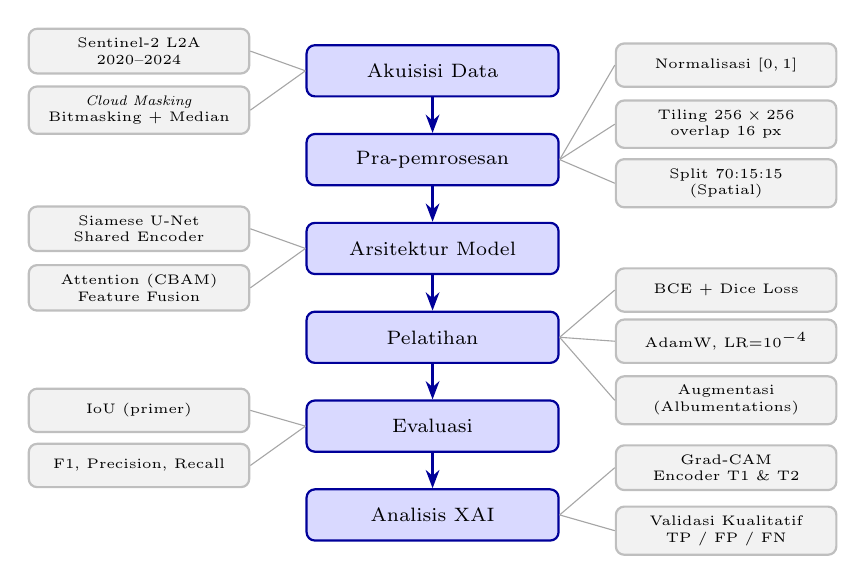
\begin{tikzpicture}[
			node distance=0.45cm,
			box/.style={
				rectangle, rounded corners=3pt,
				minimum width=3.2cm, minimum height=0.65cm,
				align=center, font=\scriptsize,
				draw, thick
			},
			mainbox/.style={box,
				fill=blue!15, draw=blue!60!black
			},
			subbox/.style={box,
				fill=gray!10, draw=gray!50,
				minimum width=2.8cm, minimum height=0.55cm,
				font=\tiny
			},
			arrow/.style={-Stealth, thick, blue!60!black},
			subarrow/.style={-, thin, gray!70},
			label/.style={font=\tiny\itshape, text=gray!70}
			]

			% --- Main pipeline (vertical center) ---
			\node[mainbox] (acq)   {Akuisisi Data};
			\node[mainbox, below=of acq]   (pre)   {Pra-pemrosesan};
			\node[mainbox, below=of pre]   (arch)  {Arsitektur Model};
			\node[mainbox, below=of arch]  (train) {Pelatihan};
			\node[mainbox, below=of train] (eval)  {Evaluasi};
			\node[mainbox, below=of eval]  (xai)   {Analisis XAI};

			% Arrows between main boxes
			\foreach \a/\b in {acq/pre, pre/arch, arch/train, train/eval, eval/xai}
			\draw[arrow] (\a) -- (\b);

			% --- Left side-notes (Akuisisi) ---
			\node[subbox, left=0.7cm of acq, yshift=0.25cm]  (s2)    {Sentinel-2 L2A\\2020--2024};
			\node[subbox, left=0.7cm of acq, yshift=-0.5cm] (mask)  {\textit{Cloud Masking}\\Bitmasking + Median};
			\draw[subarrow] (s2.east)   -- (acq.west);
			\draw[subarrow] (mask.east) -- (acq.west);

			% --- Right side-notes (Pra-pemrosesan) ---
			\node[subbox, right=0.7cm of pre, yshift=1.2cm]  (norm)  {Normalisasi $[0,1]$};
			\node[subbox, right=0.7cm of pre, yshift=0.45cm](tile)  {Tiling $256\times256$\\overlap 16 px};
			\node[subbox, right=0.7cm of pre, yshift=-0.3cm] (split) {Split 70:15:15\\(Spatial)};
			\draw[subarrow] (pre.east) -- (norm.west);
			\draw[subarrow] (pre.east) -- (tile.west);
			\draw[subarrow] (pre.east) -- (split.west);

			% --- Left side-notes (Arsitektur) ---
			\node[subbox, left=0.7cm of arch, yshift=0.25cm]  (siamese) {Siamese U-Net\\Shared Encoder};
			\node[subbox, left=0.7cm of arch, yshift=-0.5cm] (attn)    {Attention (CBAM)\\Feature Fusion};
			\draw[subarrow] (siamese.east) -- (arch.west);
			\draw[subarrow] (attn.east)    -- (arch.west);

			% --- Right side-notes (Pelatihan) ---
			\node[subbox, right=0.7cm of train, yshift=0.6cm]  (loss)  {BCE + Dice Loss};
			\node[subbox, right=0.7cm of train, yshift=-0.05cm](opt)   {AdamW, LR=$10^{-4}$};
			\node[subbox, right=0.7cm of train, yshift=-0.8cm] (aug)   {Augmentasi\\(Albumentations)};
			\draw[subarrow] (train.east) -- (loss.west);
			\draw[subarrow] (train.east) -- (opt.west);
			\draw[subarrow] (train.east) -- (aug.west);

			% --- Left side-notes (Evaluasi) ---
			\node[subbox, left=0.7cm of eval, yshift=0.2cm]  (iou) {IoU (primer)};
			\node[subbox, left=0.7cm of eval, yshift=-0.5cm] (f1)  {F1, Precision, Recall};
			\draw[subarrow] (iou.east) -- (eval.west);
			\draw[subarrow] (f1.east)  -- (eval.west);

			% --- Right side-notes (XAI) ---
			\node[subbox, right=0.7cm of xai, yshift=0.6cm]  (gc)   {Grad-CAM\\Encoder T1 \& T2};
			\node[subbox, right=0.7cm of xai, yshift=-0.2cm] (qual) {Validasi Kualitatif\\TP / FP / FN};
			\draw[subarrow] (xai.east) -- (gc.west);
			\draw[subarrow] (xai.east) -- (qual.west);

		\end{tikzpicture}
		\end{center}
	\end{frame}
	\begin{frame}
		\frametitle{Explainable AI: Grad-CAM (1)}
		
		\begin{columns}[T]
			
			\column{0.5\textwidth}
			\begin{block}{Cara Kerja}
				\small
				Grad-CAM menghitung bobot kepentingan tiap
				\textit{feature map} via \textit{global average pooling}
				atas gradien \footfullcite{DBLP:journals/corr/SelvarajuDVCPB16}:
				\[
				\alpha^c_k = \frac{1}{Z}\sum_i\sum_j
				\frac{\partial y^c}{\partial A^k_{ij}}
				\]
				\textit{Heatmap} diperoleh dari kombinasi linear
				terbobot yang dilewatkan ReLU:
				\[
				L^c_{\text{Grad-CAM}} = 
				\text{ReLU}\!\left(\sum_k \alpha^c_k A^k\right)
				\]
			\end{block}
			
			\vspace{0.2cm}
			
			\column{0.48\textwidth}
			\begin{center}
				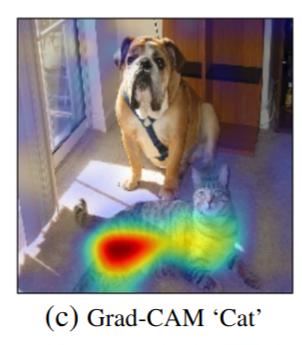
\includegraphics[width=\linewidth]{images/cat_scan.png}\\
				\vspace{0.15cm}
			\end{center}
			
			
		\end{columns}
	\end{frame}
	
	\begin{frame}
		\frametitle{Explainable AI: Grad-CAM (2)}
		\begin{alertblock}{Analisis pada 3 Kategori}
			\scriptsize
			\begin{itemize}
				\item \textbf{TP}: verifikasi fokus model
				\item \textbf{FP}: identifikasi artefak
				(awan, lahan basah)
				\item \textbf{FN}: deforestasi yang terlewat
			\end{itemize}
		\end{alertblock}
		
		\begin{block}{Mengapa Grad-CAM?}
			\small
			\begin{itemize}
				\item \textit{Class-discriminative}: membedakan
				region antar kelas \footfullcite{DBLP:journals/corr/SelvarajuDVCPB16}
				\item Tidak memerlukan perubahan arsitektur
				\item Efisien: satu \textit{forward} + satu
				\textit{backward pass}
			\end{itemize}
		\end{block}
	\end{frame}
	
	\begin{frame}[allowframebreaks]
		\frametitle{Hasil yang Diharapkan}
		
		\begin{columns}[T, onlytextwidth]
			
			\column{0.48\textwidth}
			\begin{block}{Performa Model}
				\small
				\begin{itemize}
					\item Siamese U-Net mampu mendeteksi 
					deforestasi pada citra Sentinel-2 
					multispektral Kalimantan
					\item Modifikasi arsitektur meningkatkan 
					IoU dibanding \textit{baseline}
					(\textit{ablation study})
					\item Peningkatan F1-Score menunjukkan 
					keseimbangan \textit{precision} 
					dan \textit{recall} yang lebih baik
				\end{itemize}
			\end{block}
			
			\column{0.48\textwidth}
			\begin{block}{Interpretabilitas}
				\small
				\begin{itemize}
					\item \textit{Heatmap} Grad-CAM 
					teraktivasi pada area perubahan 
					spektral nyata (penurunan NDVI, 
					peningkatan SWIR)
					\item Model tidak teraktivasi pada 
					artefak seperti awan atau 
					bayangan
					\item Analisis FP dan FN memberikan 
					wawasan untuk pengembangan 
					model lebih lanjut
				\end{itemize}
			\end{block}
			
		\end{columns}	
	\end{frame}
	
	% ─────────────────────────────────────────────────────────────
	
	\begin{frame}[allowframebreaks]
		\frametitle{Kesimpulan}
		
		\begin{block}{Pendekatan Penelitian}
			\small
			Penelitian ini menggunakan pendekatan 
			\textbf{kuantitatif} dengan elemen 
			kualitatif pada analisis XAI untuk menguji hipotesis 
			secara numerik melalui metrik segmentasi dan 
			memverifikasi interpretabilitas model via Grad-CAM
			\footfullcite{DBLP:journals/corr/SelvarajuDVCPB16}.
		\end{block}
		
		
		\begin{columns}[T]
			
			\column{0.48\textwidth}
			\begin{block}{Data}
				\small
				\begin{itemize}
					\item Citra Sentinel-2 Level-2A 
					via Google Earth Engine
					\item Label dari Hansen Global 
					Forest Change (\textit{lossyear})
					\item Wilayah studi: Kalimantan
				\end{itemize}
			\end{block}
			
			\column{0.48\textwidth}
			\begin{block}{Evaluasi}
				\small
				\begin{itemize}
					\item Metrik primer: IoU
					\item Metrik sekunder: F1, 
					Precision, Recall
					\item \textit{Ablation study} 
					antar varian arsitektur
					\item Analisis kualitatif 
					via Grad-CAM (TP, FP, FN)
				\end{itemize}
			\end{block}
			
		\end{columns}
		
		\begin{alertblock}{Kontribusi yang Diharapkan}
			\small
			Siamese U-Net yang efisien dan interpretabel 
			untuk pemantauan deforestasi Kalimantan 
			berbasis citra multispektral Sentinel-2.
		\end{alertblock}
		
	\end{frame}

	% Thanks
	\begin{frame}
		\begin{center}
				\vspace{0.15cm}
				\Huge\textit{Terima Kasih!}
		\end{center}
	\end{frame}
\end{document}